\begin{figure}
	\centering
		
	\begin{minipage}{0.65\linewidth}		
		\centering
		
		\begin{minipage}{0.5\linewidth}
			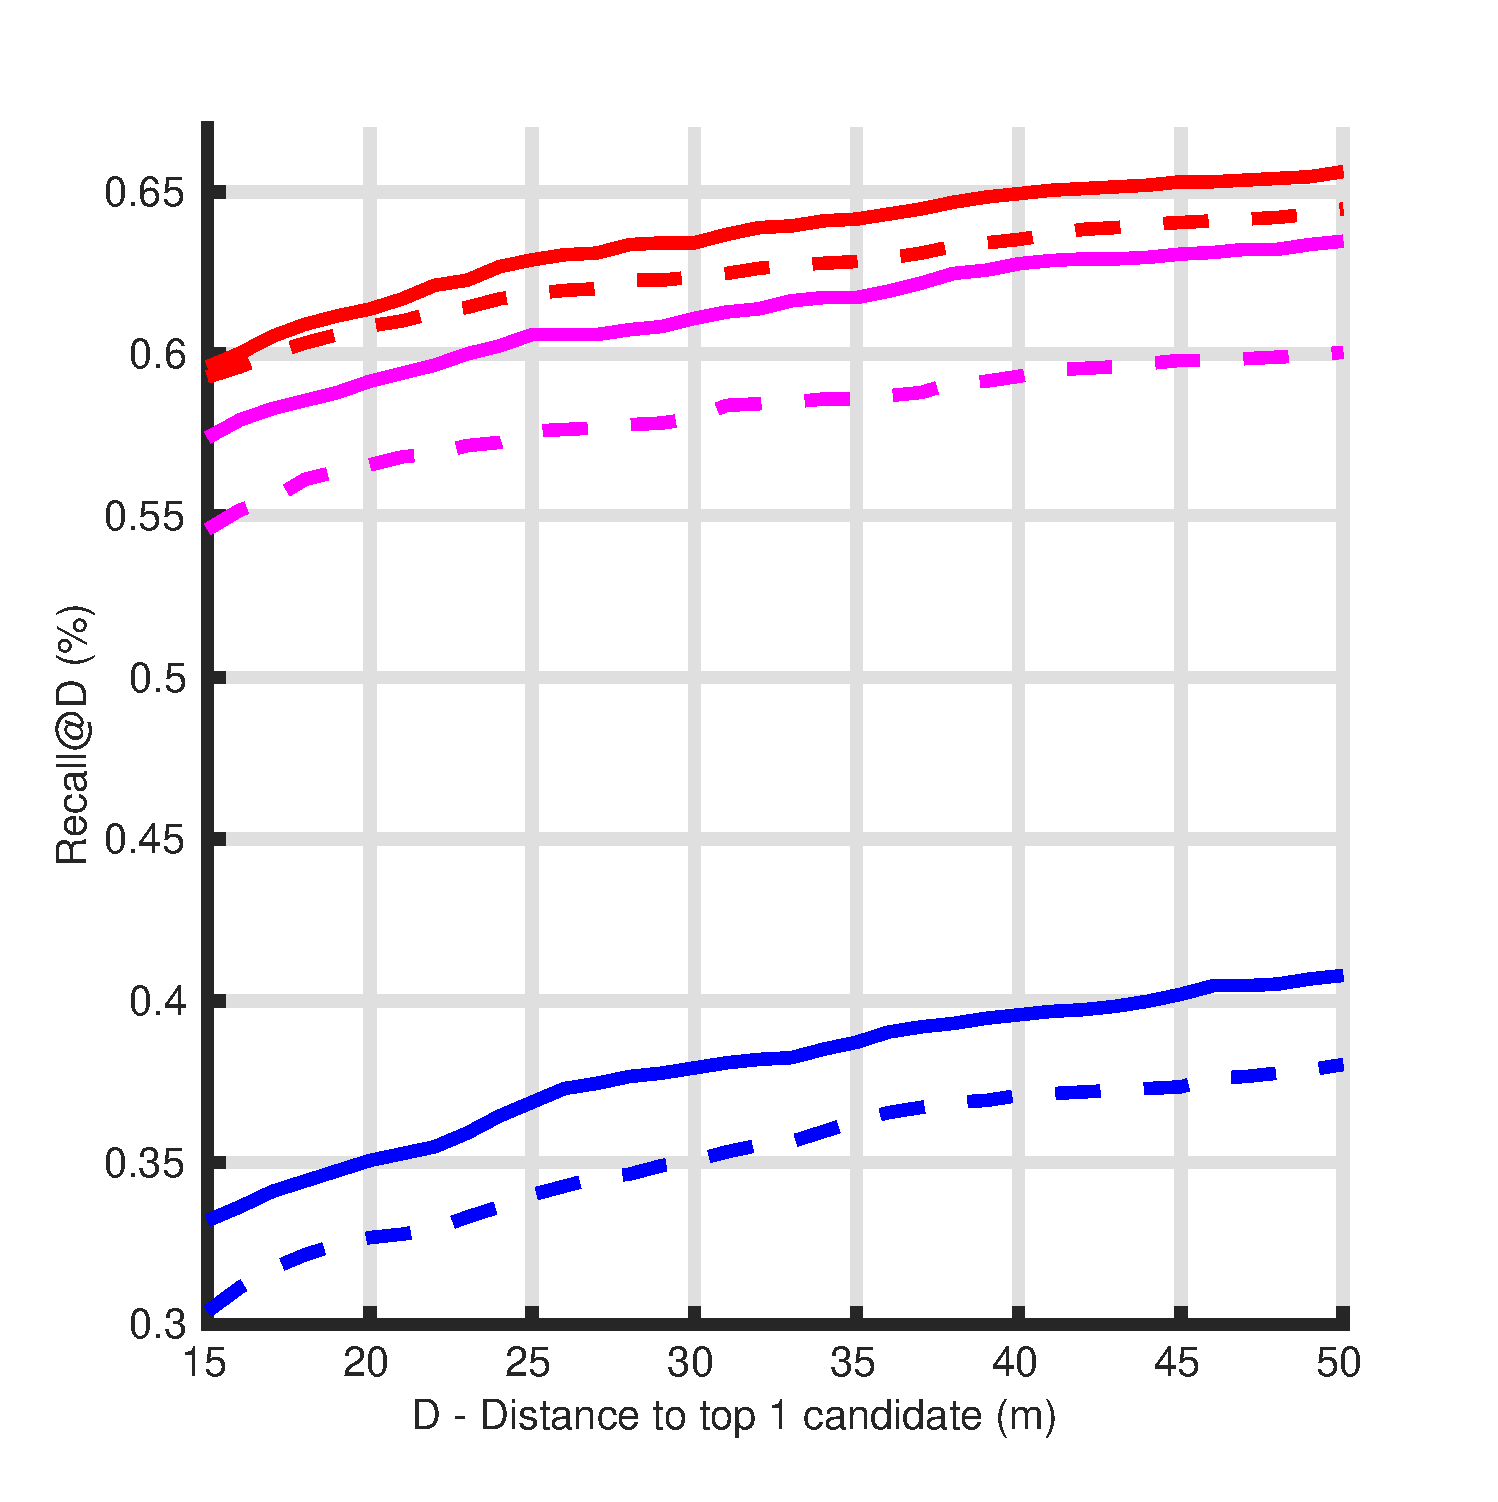
\includegraphics[width=\linewidth]{preliminary/joint_distance}
		\end{minipage}\hfill
		\begin{minipage}{0.5\linewidth}
			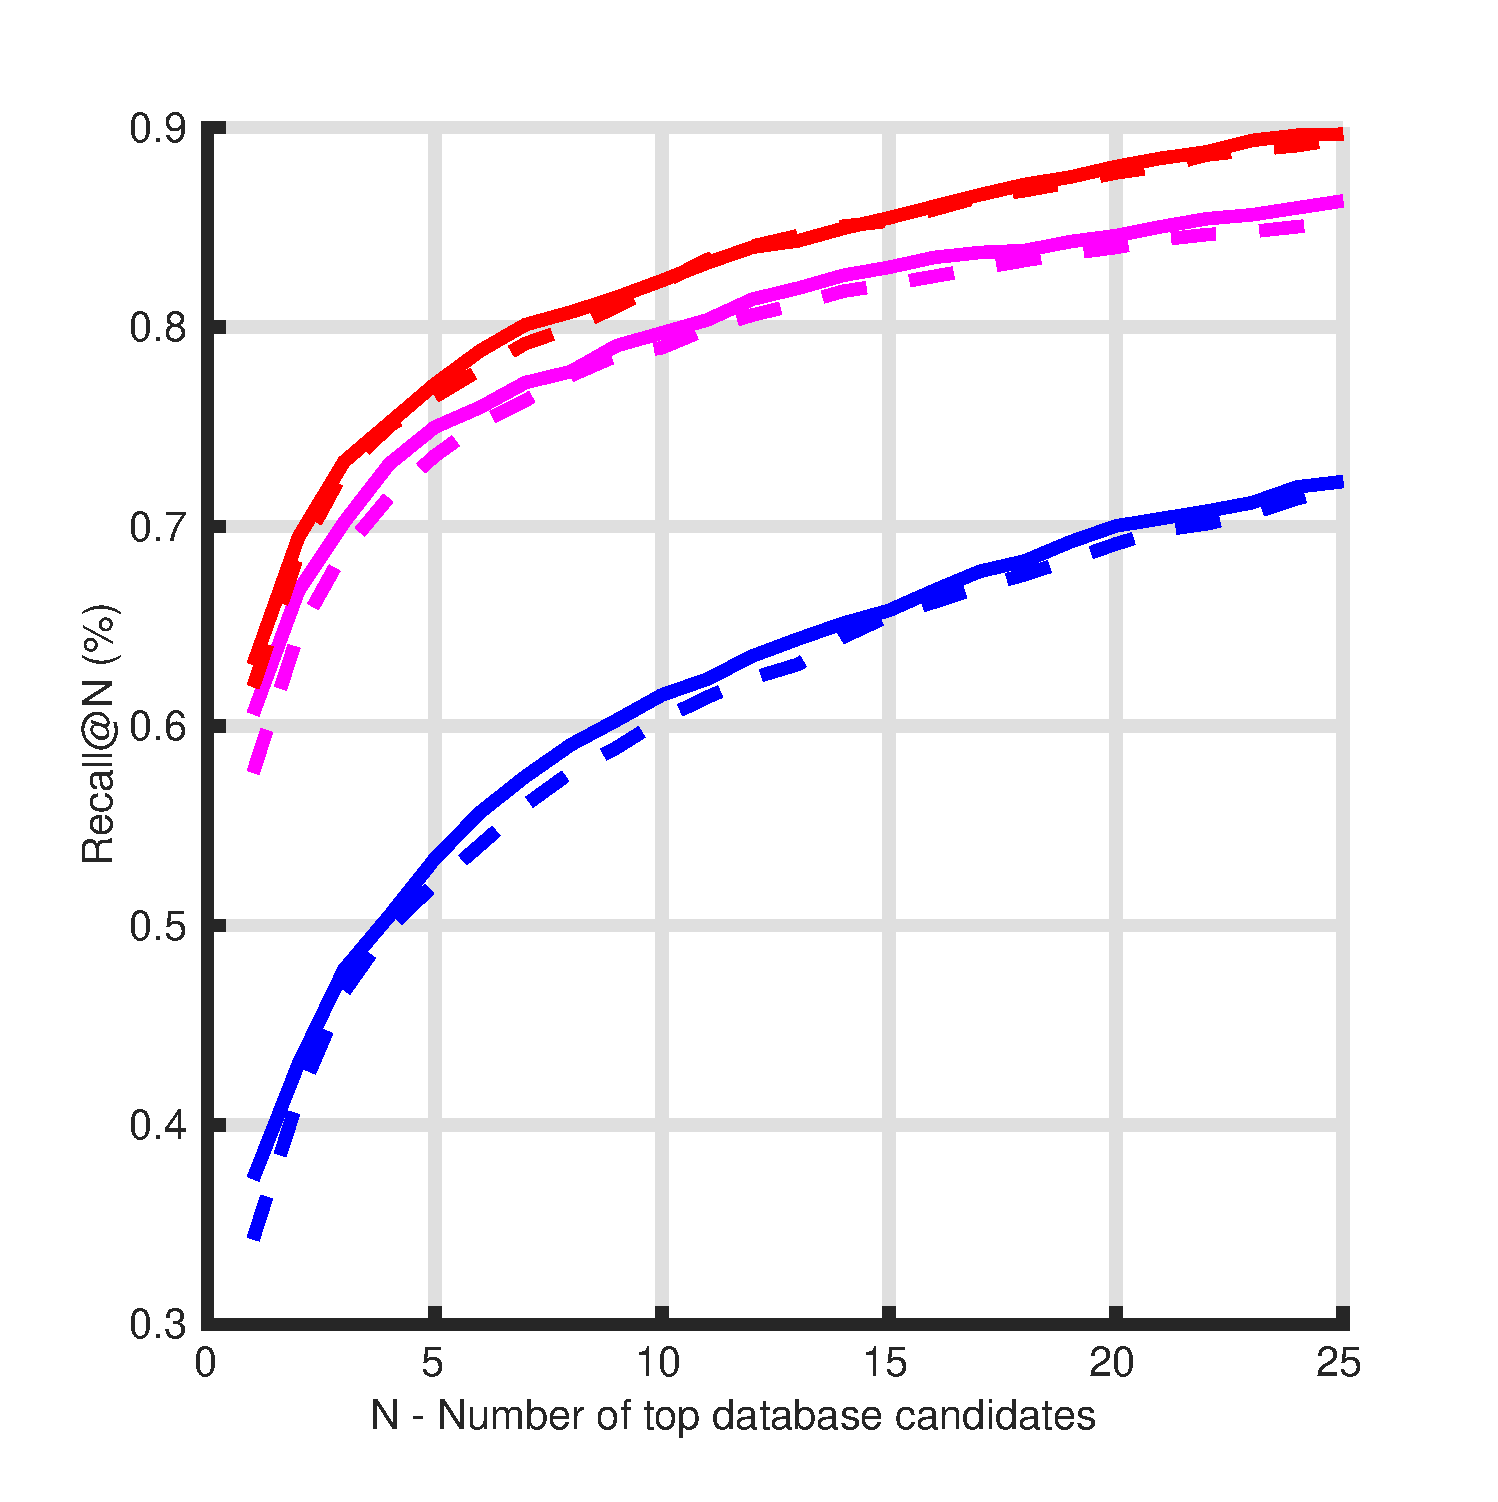
\includegraphics[width=\linewidth]{preliminary/joint_recall}
		\end{minipage}
		
		\vspace{0.2cm}
		
			\setlength{\tabcolsep}{2pt}
			\begin{tabular}{c l c l}
				\Large{- -} & Individual optimization & \textbf{\Large{--}} & Joint optimization \\
			\end{tabular}			
			
			\begin{tabular}{c c c c}
				Test set: & \textcolor{red}{{--} CMU--LT} & \textcolor{magenta}{{--} CMU--Autumn} & \textcolor{blue}{{--} CMU--Snow} \\
			\end{tabular}			
		
	\end{minipage}\hfill
	\begin{minipage}{0.35\linewidth}
		\caption[Joint vs individual optimization]{\label{fig:fuse_desc} \textbf{Influence of the joint loss $L_{p,a}$:} we report localization results of our method trained with or without the joint triplet ranking loss $L_{p,a}$. We detail the used metrics and datasets in section~\ref{sec:impl_details}.}
	\end{minipage}	

\end{figure}
	